\documentclass[letterpaper, 10 pt, conference]{ieeeconf}  % Comment this line out
                                                          % if you need a4paper
%\documentclass[a4paper, 10pt, conference]{ieeeconf}      % Use this line for a4
                                                          % paper

\IEEEoverridecommandlockouts                              % This command is only
                                                          % needed if you want to
                                                          % use the \thanks command
\overrideIEEEmargins
% See the \addtolength command later in the file to balance the column lengths
% on the last page of the document

% This is needed to prevent the style file preventing citations from linking to 
% the bibliography
\makeatletter
\let\NAT@parse\undefined
\makeatother

\usepackage[dvipsnames]{xcolor}

\newcommand*\linkcolours{ForestGreen}

\usepackage{times}
\usepackage{graphicx}
\usepackage{amssymb}
\usepackage{gensymb}
\usepackage{amsmath}
\usepackage{bbm}
\usepackage{breakurl}
\def\UrlBreaks{\do\/\do-}
\usepackage{url,hyperref}
\hypersetup{
colorlinks,
linkcolor=\linkcolours,
citecolor=\linkcolours,
filecolor=\linkcolours,
urlcolor=\linkcolours}

\usepackage{algorithm}
\usepackage{algorithmic}

\usepackage[labelfont={bf},font=small]{caption}
\usepackage[none]{hyphenat}

\usepackage{mathtools, cuted}

\usepackage[noadjust, nobreak]{cite}
\def\citepunct{,\,} % Style file defaults to listing references separately

\usepackage{tabularx}
\usepackage{amsmath}

\usepackage{float}

\usepackage{pifont}% http://ctan.org/pkg/pifont
\newcommand{\cmark}{\ding{51}}%
\newcommand{\xmark}{\ding{55}}%

\newcommand*\diff{\mathop{}\!\mathrm{d}}
\newcommand*\Diff[1]{\mathop{}\!\mathrm{d^#1}}
\newcommand*\imgres{600}

\newcolumntype{Y}{>{\centering\arraybackslash}X}

\usepackage[]{placeins}


\newcommand\extraspace{3pt}

\usepackage{placeins}

\usepackage{tikz}
\newcommand*\circled[1]{\tikz[baseline=(char.base)]{
            \node[shape=circle,draw,inner sep=0.8pt] (char) {#1};}}

\usepackage[framemethod=tikz]{mdframed}

\usepackage{afterpage}

\usepackage{stfloats}

\usepackage{atbegshi}
\newcommand{\handlethispage}{}
\newcommand{\discardpagesfromhere}{\let\handlethispage\AtBeginShipoutDiscard}
\newcommand{\keeppagesfromhere}{\let\handlethispage\relax}

% New commands added by stephen
\newcommand{\norm}[1]{\left\lVert#1\right\rVert}

\AtBeginShipout{\handlethispage}

\usepackage{comment}

% The following packages can be found on http:\\www.ctan.org
%\usepackage{graphics} % for pdf, bitmapped graphics files
%\usepackage{epsfig} % for postscript graphics files
%\usepackage{mathptmx} % assumes new font selection scheme installed
%\usepackage{times} % assumes new font selection scheme installed
%\usepackage{amsmath} % assumes amsmath package installed
%\usepackage{amssymb}  % assumes amsmath package installed

\title{\LARGE \bf
Regression-based Digit Classification on the MNIST Dataset
}

\author{Stephen Jonany$^{1}$ % <-this % stops a space
\thanks{$^{1}$Stephen is a Master's student in Applied Mathematics at the 
University of Washington.
Email: sjonany@uw.edu}%
}

\begin{document}


\maketitle
\thispagestyle{empty}
\pagestyle{empty}


%%%%%%%%%%%%%%%%%%%%%%%%%%%%%%%%%%%%%%%%%%%%%%%%%%%%%%%%%%%%%%%%%%%%%%%%%%%%%%%%
\begin{abstract}
We apply three different regression-based approaches to classify handwritten digits from the MNIST dataset, and compare their performances. The results show that simple regression-based approaches are able to achieve over 85\% accuracy, hence attesting to the usefulness of simple models.

\end{abstract}

%%%%%%%%%%%%%%%%%%%%%%%%%%%%%%%%%%%%%%%%%%%%%%%%%%%%%%%%%%%%%%%%%%%%%%%%%%%%%%%%
\section{Introduction and Overview}
Classification of handwritten digits is a classic task that has been used for benchmarking different machine learning approaches, with the MNIST dataset\cite{lecun1998mnist} being one of the most popular datasets. We explore three regression-based approaches: Lasso\cite{tibshirani1994lasso}, Ridge Regression\cite{hoerl1970ridge}, and Elastic Net\cite{zou2005elasticnet}, perform cross-validation to optimize the regularization hyperparameters and conduct feature selection by testing model performances under varying constraints of the number of pixels used as features. The test accuracy scores were over 85\%, hence showing that simple regression-based approaches appear to perform quite well on this classification task.

%%%%%%%%%%%%%%%%%%%%%%%%%%%%%%%%%%%%%%%%%%%%%%%%%%%%%%%%%%%%%%%%%%%%%%%%%%%%%%%%
\section{Theoretical Background}
\subsection{Digit Classification Task}
In the MNIST digit classification task, we are provided with a 28 x 28 2D grayscale image, where each pixel value ranges from 0 to 255, and we are asked to output a single integer ranging from 0 to 9, our best guess of the number the handwritten image is supposed to represent. A commonly used performance metric is the classification accuracy.

\begin{equation}
Accuracy =  \frac{1}{N} \sum_{i=1}^{N} \mathbbm{1}(f(x_i) = y_i).
\label{eq:accuracy}
\end{equation}
Where $N$ is the number of samples, $x_i$ is a 2D image, $y_i$ is the true digit label, and $f$ is the classification model, the accuracy measure captures the average number of data points that are classified correctly.

\subsection{Regression}
In contrast to classification tasks, where the model is asked to choose from a discrete set of options, a regression model instead outputs continuous values. We focus on the linear regression problem, where the output is a linear combination of the model parameters and the input features, as posed below.
\begin{equation}
AX = B \label{eq:regression}
\end{equation}
In this case, the data being provided are $A$, the feature matrix, and $B$, the output labels. The $X$ matrix is the linear model that we are asked to optimize.

An optimization problem is ill-defined without a concrete objective function. A common objective function for regression problems is the mean-squared error. For our linear regression formulation, we are then asked to find the model that minimizes the following objective function.
\begin{equation}
    \frac{1}{MN}\norm{AX - B}_2 \label{eq:mse}
\end{equation}
Where we assume that $B$ has $M$ rows and $N$ columns, we are penalizing the model's performance based on the Frobenius norm of the discrepancy between the model's predictions $AX$ and the true labels $B$. One possible formulation of linear regression is then to find $argmin_X \norm{AX - B}_2$.

\subsection{Regression for Digit Classification}
\label{section:regression_for_classification}
There are two questions to address before we can use regression for digit classification. First, how does one convert a collection of 2D images into a format that is acceptable for regression? Second, how does one use regression, which is purposed for a continuous-valued output, for a classification task, whose output is discrete? Finally, given the output from a regression model, how does one obtain the predicted digit?

Each 28x28 2D image is first flattened into a vector of 784 elements, where all the rows are concatenated in increasing row order. Then, all the flattened image vectors are concatenated together row-by-row to form the $A$ matrix.

Each digit label, which is a single integer ranging from 0 to 9, is converted into a vector of size 10, where the entries are all 0, except for the zero-indexed position corresponding to the digit being set to 1. That is, if the digit is 9, then the corresponding transformed vector is a 10D vector which has all 0s, except for the 10th position being set to 1. These 10D vectors are then concatenated together row-by-row to form the $B$ matrix.

To be concrete, given that the MNIST training dataset has 60,000 entries, then the entities from equation \ref{eq:regression} are now as follows:
\begin{itemize}
    \item $A$ has 60,000 rows and 784 columns, where each row corresponds to a flattened image of 784 pixels.
    \item $B$ has 60,000 rows and 10 columns, where each row has a single 1 value to indicate the true digit label, and 0 values for the rest of the indices.
    \item $X$, the model, has 784 rows and 10 columns.
\end{itemize}
This is an overdetermined system, since we have many more rows than columns.

Finally, given a 10D regression output vector, we obtain the predicted digit, by finding the index whose value is closest to 1. That is, letting $v$ be the 10D zero-indexed vector, the predicted digit is $argmin_i {|v_i - 1|}$. Now that we have described the problem transformation, we can use the classification accuracy metric described in \ref{eq:accuracy} to assess the performance of the regression model.

\subsection{Intuition behind Regression-based classification}
The interpretation behind this formulation is that we are trying to discover a latent low-dimensional structure between the image pixels and the true digit label. The 10D output vector can be thought of as the probabilities of the image corresponding to a particular digit. Because each probability value is just a linear combination of a column from $X$, the model, and a row from $A$, the flattened images, each column of $X$ can be thought of as an encoding of how different pixel intensities encode the likelihood of a particular digit. This makes an intuitive sense, since every digit has different distributions of pixel representations, just like how the digit 0 would likely not have a black pixel in the middle. 

\subsection{Regularization}
\label{section:bg-regularization}
Obtaining the model $X$ by simply minimizing the mean-squared error as described in \ref{eq:mse} is dangerous if we do not believe that our dataset is complete (which is almost always the case in practice). The resulting model would be overfit to the training data, and might fail to generalize to the test data. One approach to discourage overfitting is to add regularization terms to the objective function. We will go through three approaches which use different regularization terms.

Ridge Regression\cite{hoerl1970ridge} penalizes the magnitude of the L2 norm of the weights. The objective function to minimize is as follows.
\begin{equation}
\norm{AX - B}_2 + \alpha \norm{X}_2
\label{eq:ridge}
\end{equation}
$\alpha$ is a hyperparameter which indicates how much weight one places on the L2 norm. The higher the $\alpha$ is, the smaller the values inside $X$ will be. 

Lasso\cite{tibshirani1994lasso} penalizes the magnitude of the L1 norm of the weights. The objective function to minimize is as follows.
\begin{equation}
\norm{AX - B}_2 + \alpha \norm{X}_1
\label{eq:lasso}
\end{equation}
$\alpha$ is a hyperparameter which indicates how much weight one places on the L1 norm. The higher the $\alpha$ is, the sparser the $X$ will be. Unlike Ridge Regression, which encourages smaller non-zero weight values, lasso encourages more sparsity, where weight values go down to exactly 0.

Elastic Net\cite{zou2005elasticnet} is a combination of both approaches, where both the L1 and L2 norms of the weights are taken into account. The objective function to minimize is as follows.
\begin{equation}
\norm{AX - B}_2 + \alpha \beta \norm{X}_1 + \alpha (1 - \beta)\norm{X}_2
\label{eq:lasso}
\end{equation}
$\alpha$ is a hyperparameter which indicates how much weight one places on the norm penalties. $\beta$ is a new term that configures the ratio of L1 to L2 penalty. The higher the $\beta$, the more Lasso-like the training process will be.

\subsection{Cross-validation for Hyperparameter Optimization}
\label{section:bg-cv}
To choose the regularization hyperparameter, we used k-fold cross-validation with k=5 on the training dataset. That is, for each hyperparameter value to try, and for each of the 5 training set splits, we train on $48,000$ images, obtain the accuracy over the remaining $12,000$, and pick the hyperparameter value that maximizes the average accuracy computed over the 5 folds. Note that for Elastic Net, we fixed $\beta$ to be $0.5$, so that all the three models only have the parameter $\alpha$ to search for. 

\subsection{Feature Selection}
\label{section:feature_selection}
A compact model that performs just as well as a complicated model is to be desired.
A natural question that arises from this line of thought is whether or not we can just a subset of the image pixels for our decision process.

To find the most important pixels for the full classification problem, a measure that we can adopt is to look at each of the 784 rows in $X$, which describe how a single pixel contributes to the digit probabilities, then select the top K rows with the highest L2 norm. A higher L2 norm, intuitively, means that the training process is willing to recruit this pixel, even at the cost of an increased regularization penalty.

\subsection{Per-digit Analysis}
\label{section:per_digit_analysis}
We repeat our analysis for each individual digit, where each task becomes a binary classification task: Is this image a digit $d$ or not? The regression problem reformulation is the same as the one described in Section \ref{section:regression_for_classification}, except that we focus on 1 digit at a time instead of 10. That is, we now have 10 regression problems, where for each digit $d$ ranging from 0 to 9, we now have the following entities.

\begin{itemize}
    \item $A$ has 60,000 rows and 784 columns, where each row corresponds to a flattened image of 784 pixels.
    \item $B$ has 60,000 rows and 1 column, where each row is 1 only if the image corresponds to a digit $d$, or 0 otherwise.
    \item $X$, the model, has 784 rows and 1 column.
\end{itemize}

$X$, the model, can be thought of as representing how each pixel contributes to the likelihood of the image corresponding to a certain digit.
For prediction, we compute $AX$, which gives you a vector of likelihoods of each sample being of the digit, then for each sample we predict a digit match only if the corresponding likelihood value is over 0.5.  

To find the most important pixels for a digit, we inspect $X$ for the top K pixel weights with the highest absolute values.

%%%%%%%%%%%%%%%%%%%%%%%%%%%%%%%%%%%%%%%%%%%%%%%%%%%%%%%%%%%%%%%%%%%%%%%%%%%%%%%%
\section{Algorithm Implementation and Development}
All the codes are written in Python. The following Python libraries are used.
\begin{itemize}
    \item SciPy is used for implementations of K-fold validation, and the three linear regression approaches: Lasso, Ridge Regression and Elastic Net.
    \item NumPy is used for efficient 2D matrix manipulations.
    \item Matplotlib is used to generate all the plots.
    \item The standard \texttt{struct} module is used for byte manipulation to read in the MNIST dataset.
\end{itemize}

Translating the mathematical formulations provided in the theoretical background section to code is straightforward, and so we invite the interested readers to refer to the code appendices for the code details.

%%%%%%%%%%%%%%%%%%%%%%%%%%%%%%%%%%%%%%%%%%%%%%%%%%%%%%%%%%%%%%%%%%%%%%%%%%%%%%%%
\section{Computational Results}
\subsection{Dataset Statistics}
The dataset comprises of two separate sets of images and labels.
The training set consists of 60,000 image-label pairs, and the test set consists of just 10,000.
Each image is a 28 x 28 2D grayscale image, where each pixel value ranges from 0 (white) to 255 (black).
Each label is a single integer ranging from 0 to 9.
The training and test dataset have roughly equal number of samples for each digit as well.

\subsection{Cross-validation for Hyperparameter Optimization}
As per our discussion of regularization in Section \ref{section:bg-regularization}, we have some hyperparameters to choose to train our model with. After fixing Elastic Net's $\beta$ to be 0.5, we are left with the hyperparameter $\alpha$, which controls the strength of the regularization penalties relative to the mean-squared error. As discussed in Section \ref{section:bg-cv}, we obtain the optimal hyperparameter values by performing 5-fold cross-validation on the training set, and  pick the hyperparameter values that maximize the average accuracy across all the 5 runs.

\begin{figure}[tb] 
\centering
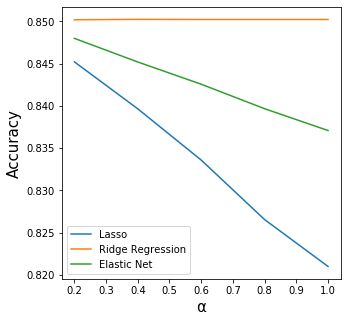
\includegraphics[width=0.97\columnwidth]{images/cv_alpha.png}
\caption{Average cross-validation classification accuracy for the three regression-based models, as $\alpha$, the hyperparameter controlling regularization weight, is varied.}
\label{fig:cv_alpha}
\end{figure}

\begin{table}[ht]
\caption{Cross-validated $\alpha$ values.} % title of Table
\centering % used for centering table
\begin{tabular}{c c c} 
\hline\hline 
Model & Best $\alpha$ & Cross-validation accuracy \% \\
\hline
Lasso & 0.2 & 84.52 \\
Ridge Regression & 0.4 & 85.03 \\
Elastic Net & 0.2 & 84.80 \\
\hline %inserts single line
\end{tabular}
\label{table:cv} % is used to refer this table in the text
\end{table}

Our results from Figure \ref{fig:cv_alpha} and Table \ref{table:cv} show that for Lasso and Elastic Net, the best $\alpha$ to use is 0.2. In fact, for these two models, increasing $\alpha$ will result in very poor cross-validation performance. Ridge Regression, on the other hand, has its highest accuracy at $\alpha = 0.4$. Interestingly enough, its performance also does not degrade as we increase $\alpha$ all the way up to $1.0$. This is perhaps because Lasso and Elastic Net, which encourages zero weights, discards many pixels from its prediction process, whereas Ridge regression still distributes its prediction process across all the pixels, albeit with smaller weights.

\subsection{Cross-validated Model Performance on Training and Test Set}
Using the cross-validated $\alpha$ values, we retrain all the models on the entire training set, and calculate both the mean-squared error as described in Equation \ref{eq:mse} and model accuracy as described in Equation \ref{eq:accuracy} on both the training and test set.

\begin{table}[ht]
\caption{Training and Test Mean-squared Error.} % title of Table
\centering % used for centering table
\begin{tabular}{c c c} 
\hline\hline 
Model & Train MSE & Test MSE \\
\hline
Lasso & 0.0003 & 0.0006 \\
Ridge Regression & 0.0003 & 0.0006  \\
Elastic Net & 0.0003 & 0.0006 \\
Linear Regression & 0.0003 & 20857.4061 \\
\hline %inserts single line
\end{tabular}
\label{table:traintest_mse_all} 
\end{table}

When we consider the mean-squared error objective function, which the regression models are optimizing for, we see that all the models are able to reach very low  mean-squared error for training. Note that the unregularized Linear Regression is the only approach with a wildly high mean-squared error on the test set, indicating that it has overfit on the training data. The other approaches that have regularization terms, on the other hand, were able to generalize well to the test data, achieving mean-squared errors that are just slightly high than the errors for the training set. 

\begin{table}[ht]
\caption{Training and Test Accuracy.} % title of Table
\centering % used for centering table
\begin{tabular}{c c c} 
\hline\hline 
Model & Train accuracy \% & Test accuracy \% \\
\hline
Lasso & 84.78 & 85.49 \\
Ridge Regression & 85.77 & \textbf{86.03} \\
Elastic Net & 85.09 & 85.75 \\
Linear Regression & \textbf{85.77} & 86.01 \\
\hline %inserts single line
\end{tabular}
\label{table:traintest_all} % is used to refer this table in the text
\end{table}

As seen in Table \ref{table:traintest_all}, the train and test accuracy of all the models hover around 85\%. Linear Regression, the only approach without any regularization, has the highest training accuracy. This is expected because the lack of regularization allows this approach to overfit on the training data.

As for the test performances, Ridge Regression performs the best, perhaps thanks to the cross-validated $\alpha$ value. Surprisingly, Linear Regression has the second best test performance, even without regularization. This might indicate that the regression problem formulation is already self-regularizing enough. Perhaps the 28x28 feature vector is already a sparse-enough feature set that it allows any regression-based classification model to generalize well to the test set distribution.

\subsection{Error Analysis}
We investigate if the classification errors can be attributed to just a few challenging digits, and if the errors could make sense even for a human. We chose to analyze the classification errors of the cross-validated Lasso model that has been trained on the full training set, and analyze its test set errors.

\begin{table*}[t]
\caption{Per-digit Test Accuracy and Confounds.} % title of Table
\centering % used for centering table
\begin{tabular}{c | c c c c c c c c c c } 
\hline\hline 

Digit & 0 & 1 & 2 & 3 & 4 & 5 & 6 & 7 & 8 & 9 \\
Accuracy \% & 96.12 & \textbf{96.92} & 79.07 & 86.73 & 89.51 & \textbf{70.29} & 91.23 & 86.19 & 77.31 & 78.89  \\
Most Confounding Digit & 6 & 8 & 1 & 7 & 9 & 3 & 0 & 1 & 1 & 7 \\
Most Confounding Error rate & 1.43 & 1.76 & 6.01 & 2.38 & 4.99 & \textbf{9.87} & 2.30 & 4.67 & 5.44 & 7.83 \\
\hline %inserts single line
\end{tabular}
\label{table:per_digit_error} % is used to refer this table in the text
\end{table*}

Table \ref{table:per_digit_error} describes the performance of the model, broken down by digit, along with the most confounding digit, and the corresponding error rate. By confounding digit, we are referring to the digit that a particular true label is most commonly mistaken for.

We see that the model is the best at classifying the number 1, with a 96.92\% chance of classifying a handwritten 1 correctly. On the other hand, the model has the hardest time identifying 5 correctly, with only a 70.29\% accuracy. In fact, in 9.87\% of the time the  model is presented with a handwritten 5, it would misclassify it as a 3.

Examples of the most confounding pairs can be seen in Figure \ref{fig:per_digit_error}. The examples of 0 being misclassified as 6 and 6 being misclassified as 0, seem reasonable enough that a human could make such a mistake. In fact, it is arguable that the image is ambiguous enough that the correct is answer is for a model to detect the ambiguity and produce two outputs instead of just one. On the other hand, the other pairs, such as when 8 is misclassified as 1, indicate that the model still has ways to go.

A disadvantage of the current linear model is that it does not capture higher-level concepts like closed loops, which a nested neural network model could be capable of detecting. Thus, it is perhaps not surprising that the model is capable of making errors that a human would think is silly.

\begin{figure*}[htp] 
\centering
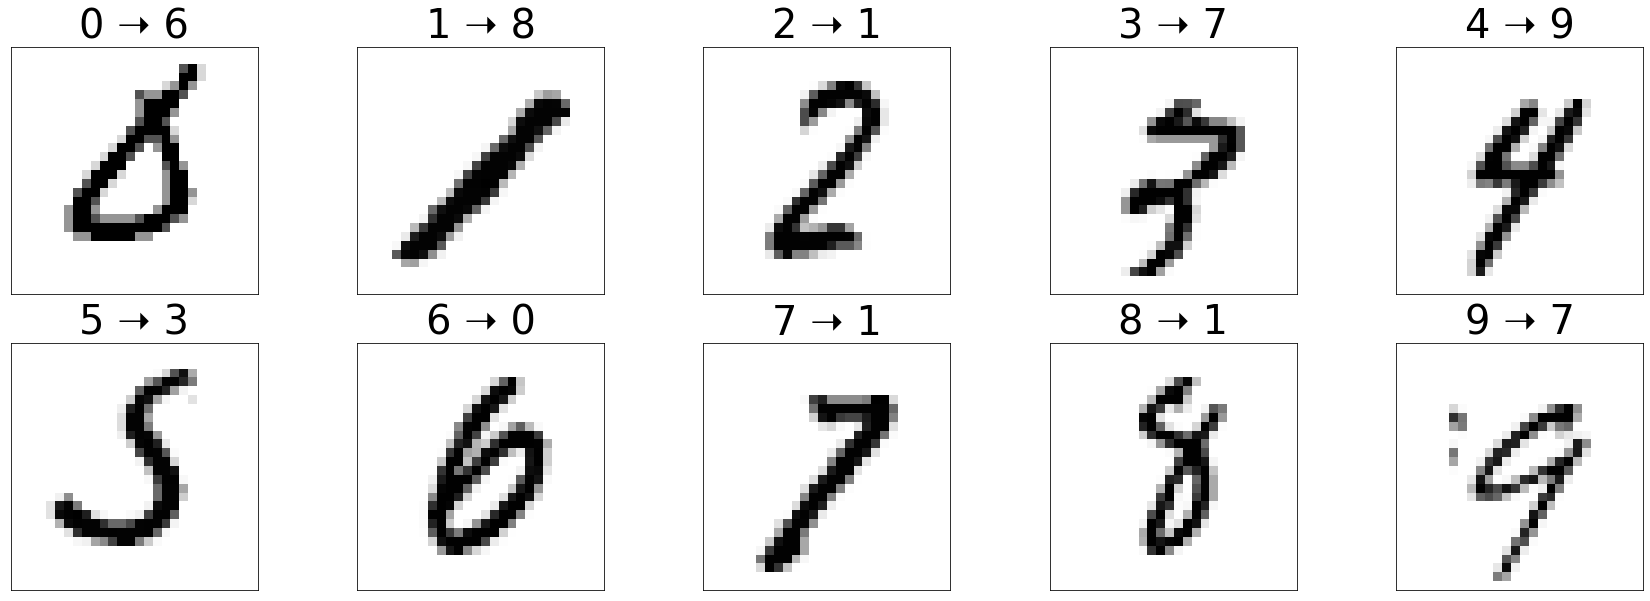
\includegraphics[width=\textwidth]{images/common_error.png}
\caption{Most common classification errors per digit. The labels above each image indicate the true label first, and the most common misidentification second. The images are the those that trigger the misclassification.}
\label{fig:per_digit_error}
\end{figure*}

\subsection{Most Important Pixels}
So far, our models have been using all 28x28 pixels for the classification process. However, as discussed in Section \ref{section:bg-cv}, we would like to see if the models can still perform reasonably well using fewer input pixels.

We look at the weight matrix of each of the three models, and subselect among the 784 rows, those with the highest L2 norms. 

\begin{figure*}[htp] 
\centering
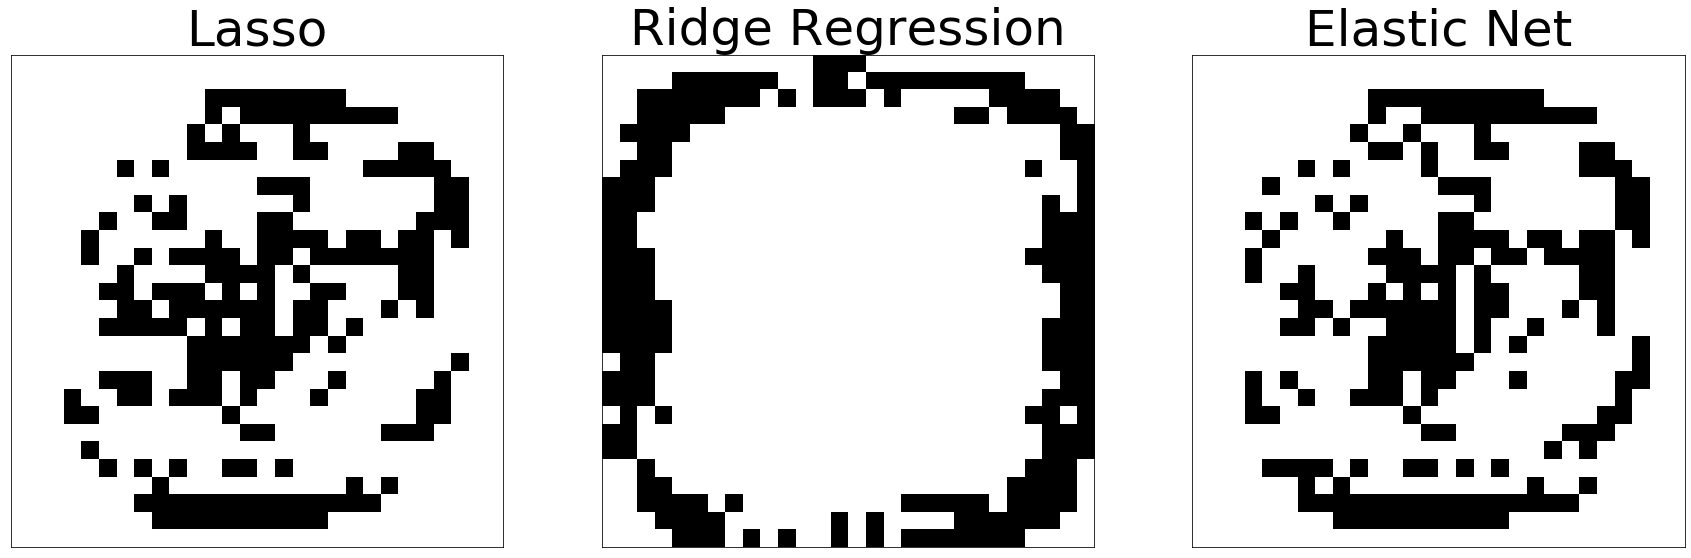
\includegraphics[width=\textwidth]{images/important_pixels_all.png}
\caption{200 pixels with the highest weight L2 norms for each approach.}
\label{fig:important_pixels_all}
\end{figure*}

As seen in Figure \ref{fig:important_pixels_all}, Lasso and Elastic Net seems to highly value the pixels around which most digits reside. One could probably see an outline of a fat 8 from the black pixels. Ridge Regression surprisingly places most of its weights on the perimeters of the image. However, we must exert caution in this comparison, because unlike Lasso and Elastic Net, which encourage 0 weights, Ridge Regression tends to keep various small weights, which are mostly non-zero. Thus, it would be unfair to assume from Figure \ref{fig:important_pixels_all} that Ridge Regression does not value the middle pixels.

\subsection{Pixel-constrained Model Performance on Test Set}
\begin{figure*}[t!] 
\centering
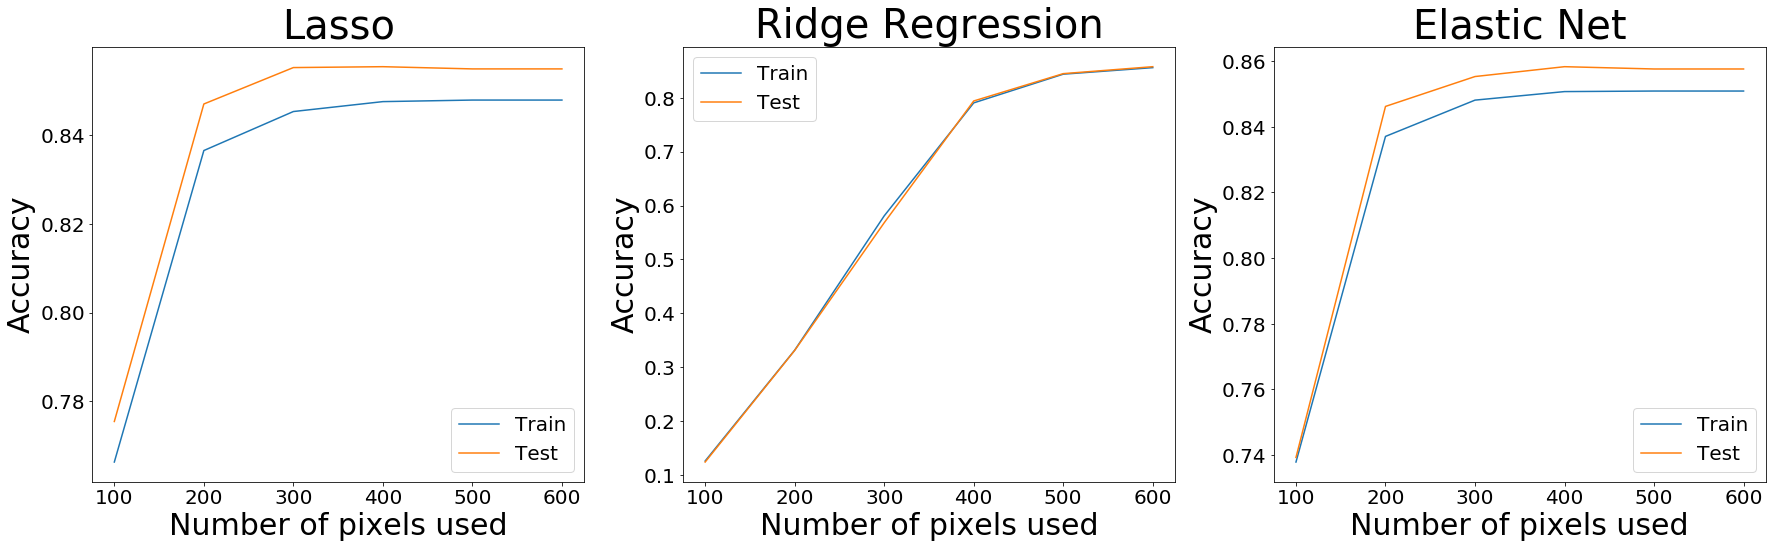
\includegraphics[width=\textwidth]{images/perf_feature_selection.png}
\caption{Training and test performance as number of pixels used is varied.}
\label{fig:perf_feature_selection}
\end{figure*}

Continuing off the previous section, we now vary the number of most important pixels to keep and measure the test performance. If the number of pixels to keep is $k$, we subsample only the top $k$ most important pixels on both train and test images. The dimensions of the regression entities from Equation \ref{eq:regression} are now as follows.
\begin{itemize}
    \item $A$ has 60,000 rows and $k$ columns, where each row corresponds to a flattened image of $k$ most important pixels.
    \item $B$ remains unchanged at 60,000 rows and 10 columns.
    \item $X$, the model, now has has $k$ rows and 10 columns.
\end{itemize}

We vary $k$, and for each value, we train each of the three models on the subsampled training data. Then, we report the model's performances on both the subsampled training and test data.

Figure \ref{fig:perf_feature_selection} shows the performances of the three models as we vary the number of input pixels allowed. As expected, the more pixels allowed, the higher the training accuracy is. It is surprising that the test performance curves resemble the training performance curves, and even outperform them. This is perhaps a sign that the hyperparameters values chosen through cross-validation have successfully prevented the model from overfitting.

Ridge Regression seems to perform the worst out of all the three models when it is constrained to use only 100 pixels. This makes sense considering that we chose the important pixels based off the weight values of the Ridge Regression model that has been trained on the full image. Since Ridge Regression does not directly encourage exactly-0 weights like Lasso does, then its decision making process is likely to be distributed over most of the pixels, making most pixels important.

As for Lasso and Elastic Net, which already encourage exactly-0 weights, throwing away pixels with the 0 weights would not affect their performances. We see that even with 100 pixels, Lasso already has a test accuracy of over 75\%, compared to Ridge Regression's measly 13\%. Furthermore, there seems to be a huge jump in accuracy, from about 75\% to 85\% as we increase the number of pixels used from 100 to 200. Increasing the number of pixels from 200 to 600 does not seem to increase the accuracy by that much, leaving us to conclude that somewhere between 100 and 200 pixels is probably the best trade off between model complexity and accuracy. 

\begin{table*}[t]
\caption{Per-digit Training and Test Accuracy.} % title of Table
\centering % used for centering table
\begin{tabular}{c | c c c c c c c c c c } 
\hline\hline 

Digit & 0 & 1 & 2 & 3 & 4 & 5 & 6 & 7 & 8 & 9 \\
Training Accuracy \% & \textbf{98.11} & 97.93 & 95.81 & 95.38 & 95.80 & 93.82 & 97.49 & 96.45 & 94.41 & \textbf{93.60}  \\
Test Accuracy \% & 97.97 & \textbf{98.04} & 95.63 & 95.60 & 96.02 & 94.11 & 97.24 & 96.45 & 94.51 & \textbf{94.02}  \\

\hline %inserts single line
\end{tabular}
\label{table:per_digit_retrain_error} % is used to refer this table in the text
\end{table*}

\begin{figure*}[t!] 
\centering
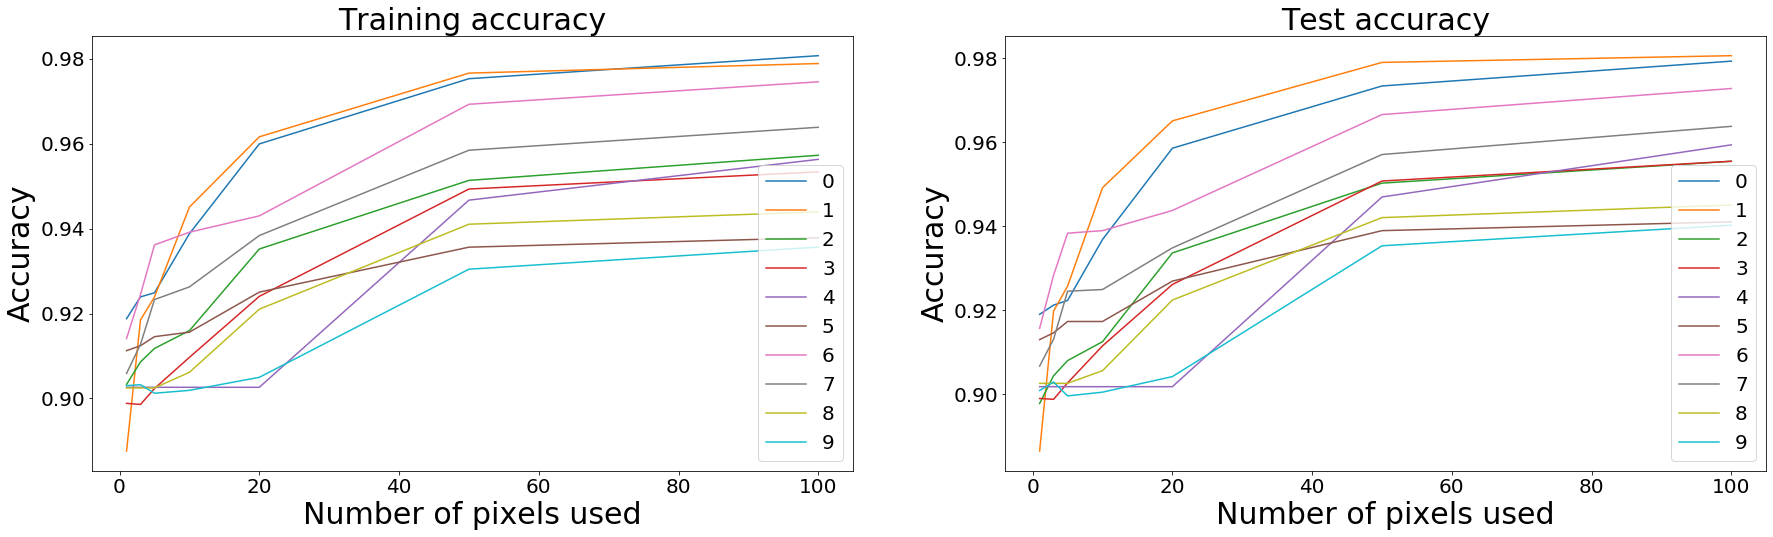
\includegraphics[width=\textwidth]{images/perf_feature_selection_per_digit.png}
\caption{For each digit, the training and test performance as number of pixels is varied.}
\label{fig:perf_feature_selection_per_digit}
\end{figure*}

\subsection{Per-Digit Binary Classification Pixel-Constrained Performance}

We repeat the same pixel-constrained analysis, but now for each digit, as described in Section \ref{section:per_digit_analysis}.

Table \ref{table:per_digit_retrain_error} shows that the per-digit binary classification task is an easier task then the 10-fold classification task, with digit 0 and 1 being the easiest to identify, with accuracies over 98\%. On the other hand, digit 9 seems to be the hardest to identify, with accuracies around 94\%.

We also vary the number of most important pixels to be used for classification, and observe the training and test accuracy. Figure \ref{fig:perf_feature_selection_per_digit} shows that we were able to reach over 90\% accuracy with less than 20 pixels. It is interesting to note that some digits, like 1, benefit greatly from additions of new pixels, whereas others, like 9, have comparably lower marginal increase in accuracy per pixel addition.

\subsection{Most Important Pixels per Digit}
\begin{figure*}[t!] 
\centering
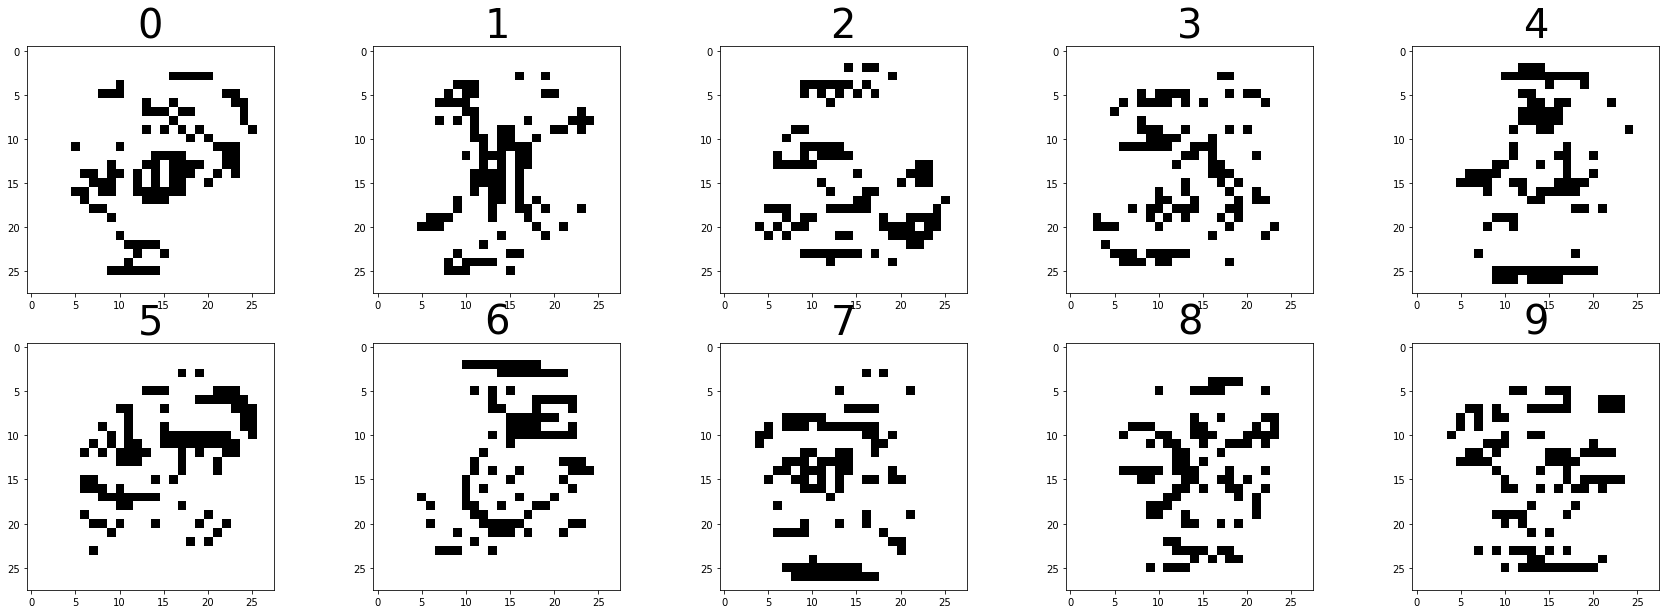
\includegraphics[width=\textwidth]{images/important_pixels_per_digit.png}
\caption{For each digit, in black are the 100 most important 100 pixels for the fully-trained Lasso model.}
\label{fig:important_pixels_per_digit}
\end{figure*}

It is interesting to see what pixels are most pivotal for the identification of each digit. As described in Section
\ref{section:per_digit_analysis}, for each digit, we consider pixels whose weight values have the highest absolute values.

For the Lasso model that has been trained on the per-digit training sets, we inspect its weight matrix for the 100 most important pixels for each digit. From Figure \ref{fig:important_pixels_per_digit}, we can see distinctive shapes for each digit, hinting that the model discovered different distributions of key pixels for distinguishing between different digits. It is worth noting that most of the important pixels are clustered near the center, which makes sense, because that is where most of the distinguishing digit features would be located.

If one were to squint, one could perhaps argue that the important pixels for the digit 3 form a vague outline of 3. However, it is unclear to derive an intuitive explanation behind the distributions of the important pixels for the other digits. 

%%%%%%%%%%%%%%%%%%%%%%%%%%%%%%%%%%%%%%%%%%%%%%%%%%%%%%%%%%%%%%%%%%%%%%%%%%%%%%%%
\section{Summary and Conclusions}
Regression is a simple but surprisingly powerful tool.
Even in the task of digit classification, where we have to reformulate the problem into a regression problem, the models are able to achieve accuracy of over 85\%. Through our feature selection experiments, we were also able to show that Lasso is not only useful for detecting the important pixels, but also perform almost as well with just 100 pixels. This highlights the utility of Lasso as a tool for balancing model complexity and accuracy. Finally, we showed that the per-digit binary classification problem is a much easier task than the 10-digit classification problem, with some digits achieving test accuracy as high as 98\%.

\bibliographystyle{ieeetr}
\bibliography{bibliography}
\clearpage

\onecolumn
%%%%%%%%%%%%%%%%%%%%%%%%%%%%%%%%%%%%%%%%%%%%%%%%%%%%%%%%%%%%%%%%%%%%%%%%%%%%%%%%
\section*{Appendix A: Key Python functions}
\subsection*{Convert MNIST matrices into the regression form $AX = B$}
\begin{verbatim}
def convert_labels_to_binary_vector(labels):
  """
  Convert the digit labels into binary arrays
  """
  labels = labels.reshape((1, len(labels)))
  binary_mat = np.zeros((labels.size, labels.max()+1))
  binary_mat[np.arange(labels.size), labels] = 1
  return binary_mat

train_flat_images = train_images.reshape(num_train_images, num_image_row * num_image_col)
test_flat_images = test_images.reshape(num_test_images, num_image_row * num_image_col)
train_binary_labels = util.convert_labels_to_binary_vector(train_labels)
test_binary_labels = util.convert_labels_to_binary_vector(test_labels)
\end{verbatim}

\subsection*{Hyperparameter optimization using K-fold cross validation}
\begin{verbatim}
def get_kfold_accuracy(model, train_flat_images, train_binary_labels, train_labels):
  num_fold = 5
  kf = KFold(n_splits=num_fold, random_state = 1, shuffle = True)
  splits = kf.split(train_flat_images)
  fold = 1
  total_acc = 0
  for train_indices, test_indices in splits:
    start_time = time.time()
    fold_train_images = train_flat_images[train_indices, :]
    fold_test_images = train_flat_images[test_indices, :]
    fold_train_binary_labels = train_binary_labels[train_indices, :]
    fold_test_labels = train_labels[test_indices]
    model.fit(fold_train_images, fold_train_binary_labels)
    preds = get_predictions(model, fold_test_images)
    errs = get_errors(preds, fold_test_labels)
    acc = get_accuracy(len(errs), len(fold_test_labels))
    print("Fold %d takes %d seconds, accuracy = %.2f" %
          (fold, time.time() - start_time, acc))
    fold += 1
    total_acc += acc
  return 1.0 * total_acc / num_fold
  
 def convert_regressed_vec_to_digit(vec):
  """
  Convert the regression result to a single digit prediction.
  We do this by finding an element that is closest to 1.
  """
  return np.argmin(np.abs(vec - 1))

def get_predictions(model, images):
  regress_vecs = model.predict(images)
  # Convert each row of regressed vector to a digt
  preds = np.apply_along_axis(convert_regressed_vec_to_digit, 1, regress_vecs)
  return preds

def get_errors(predictions, labels):
  return np.argwhere(labels != predictions).flatten()

def get_accuracy(num_error, num_samples):
  return 1.0 * (num_samples - num_error ) / num_samples

lasso_alpha_to_acc = {}
alphas = [0.2, 0.4, 0.6, 0.8, 1.0]
for alpha in alphas:
  if alpha in lasso_alpha_to_acc:
    continue
  model = linear_model.Lasso(alpha=alpha)
  acc = util.get_kfold_accuracy(model, train_flat_images, train_binary_labels, train_labels)
  print("For alpha = %.2f, accuracy for Lasso = %.2f" % (alpha, acc))
  lasso_alpha_to_acc[alpha] = acc
# Optimize ridge regression's hyperparameter.
ridge_alpha_to_acc = {}
for alpha in alphas:
  if alpha in ridge_alpha_to_acc:
    continue
  model = linear_model.Ridge(alpha=alpha)
  acc = util.get_kfold_accuracy(model, train_flat_images, train_binary_labels, train_labels)
  print("For alpha = %.2f, accuracy for Ridge = %.2f" % (alpha, acc))
  ridge_alpha_to_acc[alpha] = acc
# Optimize elastic net's hyperparameters.
elastic_alpha_to_acc = {}
for alpha in alphas:
  if alpha in elastic_alpha_to_acc:
    continue
  model = linear_model.ElasticNet(alpha=alpha,l1_ratio=0.5)
  acc = util.get_kfold_accuracy(model, train_flat_images, train_binary_labels, train_labels)
  print("For alpha = %.2f, accuracy for Elastic net = %.2f" % (alpha, acc))
  elastic_alpha_to_acc[alpha] = acc
\end{verbatim}

\subsection*{Compute accuracy and mean-squared error on training and test set}
\begin{verbatim}
best_lasso_alpha = 0.2
best_ridge_alpha = 0.4
best_elastic_alpha = 0.2

best_lasso = linear_model.Lasso(alpha=best_lasso_alpha)
best_ridge = linear_model.Ridge(alpha=best_ridge_alpha)
best_elastic = linear_model.ElasticNet(alpha=best_elastic_alpha, l1_ratio=0.5)
plain_regression = linear_model.LinearRegression()

def get_model_train_test_performance(model, model_name):
  model.fit(train_flat_images, train_binary_labels)
  model_train_preds = util.get_predictions(model, train_flat_images)
  model_train_errs = util.get_errors(model_train_preds, train_labels)
  model_train_acc = util.get_accuracy(len(model_train_errs), num_train_images)
  model_test_preds = util.get_predictions(model, test_flat_images)
  model_test_errs = util.get_errors(model_test_preds, test_labels)
  model_test_acc = util.get_accuracy(len(model_test_errs), num_test_images)
  print("%s. Train accuracy = %.4f. Test accuracy = %.4f" % \
        (model_name, model_train_acc, model_test_acc))
  return model_test_preds
lasso_test_preds = get_model_train_test_performance(best_lasso, "Lasso")
get_model_train_test_performance(best_ridge, "Ridge Regression")
get_model_train_test_performance(best_elastic, "Elastic Net")
get_model_train_test_performance(plain_regression, "Linear Regression")

def get_mse(model, flat_images, binary_labels):
  # Return the L2 norm of AX - b
  predicted_b = model.predict(flat_images)
  num_els = predicted_b.shape[0] * predicted_b.shape[1]
  mse = 1.0 / num_els * LA.norm(predicted_b - binary_labels)
  return mse

def get_model_train_test_mse(model, model_name):
  train_mse = get_mse(model, train_flat_images, train_binary_labels)
  test_mse = get_mse(model, test_flat_images, test_binary_labels)
  
  print("%s. Train MSE = %.4f. Test MSE = %.4f" % \
        (model_name, train_mse, test_mse))
get_model_train_test_mse(best_lasso, "Lasso")
get_model_train_test_mse(best_ridge, "Ridge Regression")
get_model_train_test_mse(best_elastic, "Elastic Net")
get_model_train_test_mse(plain_regression, "Linear Regression")
\end{verbatim}

\subsection*{Error analysis to find the confounding digit pairs}
\begin{verbatim}
actual_to_predicted_counts = np.zeros((10, 10), dtype=int)
actual_to_predicted_sample = np.zeros((10, 10), dtype=int)
for i in range(len(lasso_test_preds)):
  pred = lasso_test_preds[i]
  actual = test_labels[i]
  actual_to_predicted_counts[actual, pred] += 1
  actual_to_predicted_sample[actual, pred] = i

digit_to_confound = {}
print("Digit, Classification accuracy, Most confounding digit, Most confounding error rate")
for digit in range(10):
  num_samples_for_digit = actual_to_predicted_counts[digit, :].sum()
  correct_preds_for_digit = actual_to_predicted_counts[digit, digit]
  digit_acc = 100.0 * correct_preds_for_digit / num_samples_for_digit 
  
  # Remove the correct prediction so we can argmax to get confounding error 
  actual_to_predicted_counts[digit, digit] = -1
  most_confounding_digit = actual_to_predicted_counts[digit, :].argmax()
  most_confounding_err_count = actual_to_predicted_counts[digit, most_confounding_digit]
  most_confounding_err_rate = 100.0 * most_confounding_err_count / num_samples_for_digit
  actual_to_predicted_counts[digit, digit] = correct_preds_for_digit
  print("%d, %.2f, %d, %.2f" % (digit, digit_acc, most_confounding_digit,
    most_confounding_err_rate))
  
  digit_to_confound[digit] = most_confounding_digit
\end{verbatim}

\subsection*{Important pixel detection}
\begin{verbatim}
# Get the L2 norm of each weight row to find most important pixels.
fig, axes = plt.subplots(nrows=1, ncols =3, figsize=(30,10))
i = 0
model_names = ["Lasso", "Ridge Regression", "Elastic Net"]
for model in [best_lasso, best_ridge, best_elastic]:
  X = model.coef_.T
  k = 200
  weight_l2 = np.apply_along_axis(LA.norm, 1, X)
  top_pixel_indices = weight_l2.argsort()[-k:][::-1]
  ax = axes[i]
  util.plot_important_pixels(ax, top_pixel_indices)
  ax.get_xaxis().set_visible(False)
  ax.set_title(model_names[i], fontsize = 50)
  ax.get_yaxis().set_visible(False)
  i+=1

# Get the most important pixels for each digit.
k = 100
fig, axes = plt.subplots(nrows=2, ncols = 5, figsize=(30,10))
for digit in range(10):
  ax_row = digit // 5
  ax_col = digit % 5
  ax = axes[ax_row][ax_col]
  weights_for_digit = np.abs(best_lasso.coef_[digit, :])
  top_pixel_indices = weights_for_digit.argsort()[-k:][::-1]
  util.plot_important_pixels(ax, top_pixel_indices)
  ax.set_title(digit, fontsize=40)
\end{verbatim}

\subsection*{Varying pixels used for per-digit classification}
\begin{verbatim}
    def get_one_digit_labels(digit, binary_labels):
  return binary_labels[:, digit]

def get_one_digit_accuracy(proba_predictions, one_digit_train_binary_labels):
  binary_predictions = proba_predictions > 0.5
  num_correct = sum(binary_predictions == one_digit_train_binary_labels)
  return 1.0 * num_correct / len(proba_predictions)
get_one_digit_labels(0, train_binary_labels)

NUM_DIGIT = 10
full_train_error_per_digit = np.zeros(NUM_DIGIT)
full_test_error_per_digit = np.zeros(NUM_DIGIT)
# list<map<pixel_count, train error>> 
partial_pixel_train_error_per_digit = [{} for x in range(NUM_DIGIT)]
# list<map<pixel_count, test error>>
partial_pixel_test_error_per_digit = [{} for x in range(NUM_DIGIT)]

model = best_lasso

top_ks = [1, 3, 5, 10, 20, 50, 100]
k = 100
fig, axes = plt.subplots(nrows=2, ncols = 5, figsize=(30,10))

for digit in range(NUM_DIGIT):
  one_digit_train_binary_labels = get_one_digit_labels(digit, train_binary_labels)
  one_digit_test_binary_labels = get_one_digit_labels(digit, test_binary_labels)
  model.fit(train_flat_images, one_digit_train_binary_labels)
  
  # This is a 1-D array, each element is like a probability that the classifier
  # thinks it's this particular digit
  train_proba_preds = model.predict(train_flat_images)
  model_train_acc = get_one_digit_accuracy(train_proba_preds, one_digit_train_binary_labels)
  test_proba_preds = model.predict(test_flat_images)
  model_test_acc = get_one_digit_accuracy(test_proba_preds, one_digit_test_binary_labels)
  
  full_train_error_per_digit[digit] = model_train_acc
  full_test_error_per_digit[digit] = model_test_acc
  
  print("Digit = %d. Train accuracy = %.4f. Test accuracy = %.4f" % \
        (digit, model_train_acc, model_test_acc))
  
  # Plot most important pixels
  ax_row = digit // 5
  ax_col = digit % 5
  ax = axes[ax_row][ax_col]
  weights_for_digit = np.abs(model.coef_)
  top_pixel_indices = weights_for_digit.argsort()[-k:][::-1]
  util.plot_important_pixels(ax, top_pixel_indices)
  ax.set_title(digit, fontsize=40)
  
  # Retrain on a subset of pixels
  for top_k in top_ks:
    start_time = time.time()
    selected_pixels = top_pixel_indices[:top_k]
    sampled_train_flat_images = util.subsample_pixels(train_flat_images, selected_pixels)
    sampled_test_flat_images = util.subsample_pixels(test_flat_images, selected_pixels)
    model.fit(sampled_train_flat_images, one_digit_train_binary_labels)
    
    train_proba_preds = model.predict(sampled_train_flat_images)
    model_train_acc = get_one_digit_accuracy(train_proba_preds, one_digit_train_binary_labels)
    test_proba_preds = model.predict(sampled_test_flat_images)
    model_test_acc = get_one_digit_accuracy(test_proba_preds, one_digit_test_binary_labels)
    
    print("Digit = %d. Top k = %d, Train accuracy = %.2f, Test accuracy = %.2f" % 
          (digit, top_k, model_train_acc, model_test_acc))
    partial_pixel_train_error_per_digit[digit][top_k] = model_train_acc
    partial_pixel_test_error_per_digit[digit][top_k] = model_test_acc
    print("This one iteration took %d s" % (time.time() - start_time))
    
def plot_varying_pixel_performance(partial_pixel_error_per_digit, ax):
  for digit in range(NUM_DIGIT):
    accs = [partial_pixel_error_per_digit[digit][top_k] for top_k in top_ks]
    ax.plot(top_ks, accs, label=str(digit))
  ax.set_xlabel("Number of pixels used")
  ax.set_ylabel("Accuracy")
  ax.set_title(model_name, fontsize=40)
  ax.xaxis.label.set_fontsize(30)
  ax.yaxis.label.set_fontsize(30)
  for tick in ax.xaxis.get_major_ticks():
    tick.label.set_fontsize(20) 
  for tick in ax.yaxis.get_major_ticks():
    tick.label.set_fontsize(20) 
  ax.legend(prop={'size': 20})
  
fig, axes = plt.subplots(nrows=1, ncols = 2, figsize=(30,8))
plot_varying_pixel_performance(partial_pixel_train_error_per_digit, axes[0])
plot_varying_pixel_performance(partial_pixel_test_error_per_digit, axes[1])
axes[0].set_title("Training accuracy", fontsize = 30)
axes[1].set_title("Test accuracy", fontsize = 30)
\end{verbatim}
%%%%%%%%%%%%%%%%%%%%%%%%%%%%%%%%%%%%%%%%%%%%%%%%%%%%%%%%%%%%%%%%%%%%%%%%%%%%%%%%
\section*{Appendix B: Supporting Python codes}
The rest of the supporting Python codes can be found on \url{https://github.com/sjonany/AMATH563-public/tree/master/hw1/code}
\end{document}